\documentclass[11pt,letterpaper]{article}
\usepackage[lmargin=1in,rmargin=1in,tmargin=1in,bmargin=1in]{geometry}
\usepackage{../style/homework}
\usepackage{../style/commands}
\setbool{quotetype}{true} % True: Side; False: Under
\setbool{hideans}{false} % Student: True; Instructor: False

% -------------------
% Content
% -------------------
\begin{document}

\homework{11: Due 05/02}{The laws of probability, so true in general, so fallacious in particular.}{Edward Gibbon}

% Problem 1
\problem{10} The probabilities of several events in a finite probability space are given below:
	\[
	\begin{aligned}
	P(A)&= 0.10 & P(A \text{ and } B)&= 0.06 \\
	P(B)&= 0.34 & P(A \text{ and } C)&= 0.77 \\
	P(C)&= 0.81 & P(B \text{ or } C)&= 0.25 \\
	P(D)&= 0.50 & P(B \text{ and } D)&= 0.00
	\end{aligned}
	\] 
\begin{enumerate}[(a)]
\item Find $P(A \text{ or } B)$. 
\item Assuming $A$ and $D$ are independent events, find $P(A \text{ and } D)$.
\item Find $P(A \;|\; B)$.
\item Find $P(B \text{ and } C)$. 
\item Are $C$ and $D$ disjoint? Explain.
\item Are $A$ and $C$ independent? Explain.
\item Are $B$ and $D$ independent? Explain.
\end{enumerate} \pspace

\sol
\begin{enumerate}[(a)]
\item 
	\[
	P(A \text{ or }B)= P(A) + P(B) - P(A \text{ and }B)= 0.10 + 0.34 - 0.06= 0.38
	\]

\item 
	\[
	P(A \text{ and }D)= P(A) \cdot P(D)= 0.10 \cdot 0.50= 0.05
	\]

\item 
	\[
	P(A \;|\; B)= \dfrac{P(A \text{ and }B)}{P(B)}= \dfrac{0.06}{0.34}= 0.1765
	\]

\item 
	\[
	\begin{aligned}
	P(B \text{ or }C)&= P(B) + P(C) - P(B \text{ and }C) \\
	0.25&= 0.34 + 0.81 - P(B \text{ and } C) \\
	P(B \text{ and } C)&= 0.90
	\end{aligned}
	\]

\item If $C$ and $D$ were disjoint, then $P(C \text{ or }D)= P(C) + P(D)= 0.81 + 0.50= 1.31 > 1$, which is impossible. Therefore, $C$ and $D$ cannot be disjoint. 

\item If $A$ and $C$ were independent, then $P(A \text{ and }C)= P(A) \cdot P(C)$. But $P(A \text{ and }C)= 0.77$ while $P(A) \cdot P(C)= 0.10 \cdot 0.81= 0.081$. Therefore, $A$ and $C$ are not independent. 

\item We see that $P(B \text{ and } D)= 0.00$. Therefore, $B$ and $D$ are disjoint. But then $B$ and $D$ cannot be independent because disjoint events are never independent. 
\end{enumerate}



\newpage



% Problem 2
\problem{10} Of the most recent hit `scamster' shows, people were surveyed about whether they had watched \textit{The Dropout} or \textit{Inventing Anna}. Fifty people were surveyed with twenty-one of them saying that they had seen \textit{The Dropout}, thirty-seven of them saying that they had seen \textit{Inventing Anna}, and twelve of them saying that they had watched both. Suppose you select one of these fifty people at random. 
	\begin{enumerate}[(a)]
	\item Find the probability that they had seen \textit{The Dropout}.
	\item Find the probability that they had only seen \textit{Inventing Anna}.
	\item Find the probability that they had seen neither show.
	\item Find the probability that they had seen \textit{The Dropout} given that they had seen \textit{Inventing Anna}.
	\end{enumerate} \pspace

\sol
\begin{enumerate}[(a)]
\item 
	\[
	\begin{aligned}
	P(\text{Dropout})= \dfrac{9 + 12}{50}= \dfrac{21}{50} \approx 0.42
	\end{aligned}
	\]

\item 
	\[
	P(\text{Only Inventing})= \dfrac{25}{50} \approx 0.50
	\]

\item 
	\[
	P(\text{Neither})= \dfrac{4}{50} \approx 0.08
	\]

\item 
	\[
	P(\text{Dropout} \;|\; \text{Inventing})= \dfrac{12}{12 + 25}= \dfrac{12}{37} \approx 0.3243
	\]
\end{enumerate} \pspace

	\[
	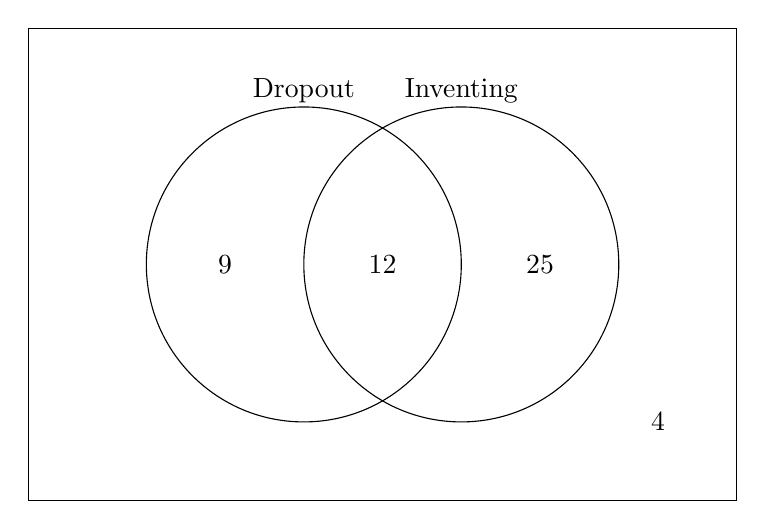
\begin{tikzpicture}
	\draw (0,0) rectangle (9,6);
	\draw (3.5,3) circle (2);
	\draw (5.5,3) circle (2);
	
	\node at (3.5,5.2) {Dropout};
	\node at (5.5,5.2) {Inventing}; 
	
	\node at (2.5,3) {9};
	\node at (4.5,3) {12};
	\node at (6.5,3) {25};
	\node at (8,1) {4};
	\end{tikzpicture}
	\]



\newpage



% Problem 3
\problem{10} Suppose a blood test for a common genetic marker correctly identifies when a person has the marker 97.4\% of the time. The test incorrectly indicates that a person has the marker when they do not 6.5\% of the time. It is estimated that 78\% of the population possesses the genetic marker. 
	\begin{enumerate}[(a)]
	\item What is the probability that a person that tests positive for the marker has the genetic marker?
	\item What is the probability that a person being tested for the marker will test positive or have the marker? 
	\item What is the probability that a person that does not possess the marker will test negative for the marker?
	\item Given that a person tests for the marker, what is the probability that they actually have the marker? 
	\end{enumerate} \pspace

\sol
\begin{enumerate}[(a)]
\item 
	\[
	P(H \;|\; +)= \dfrac{0.75972}{0.75972 + 0.0143}= \dfrac{0.75972}{0.77402}= 0.981525
	\] \pspace

\item 
	\[
	P(+ \text{ or } H)= 0.75972 + 0.02028 + 0.0143= 0.7943
	\] \pspace

\item 
	\[
	P(- \;|\; N)= \dfrac{0.2057}{0.0143 + 0.2057}= \dfrac{0.2057}{0.22}= 0.935
	\] \pspace

\item 
	\[
	P(H \;|\; +)= \dfrac{0.75972}{0.75972 + 0.0143}= \dfrac{0.75972}{0.77402}= 0.981525
	\]
\end{enumerate} \pspace

		\[
		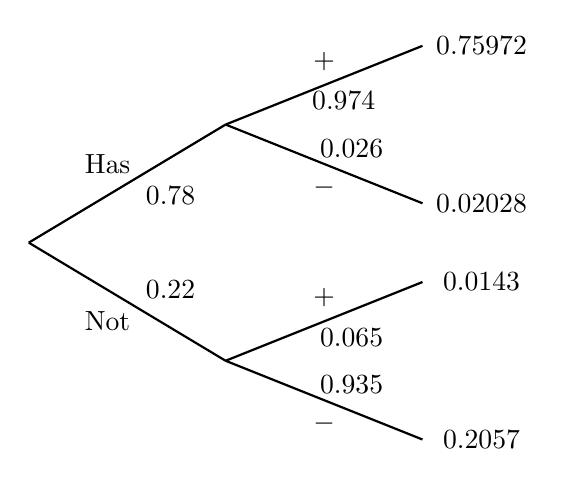
\begin{tikzpicture}[scale= 1.0]
		\def\FirstUpLabel{Has}
		\def\FirstDownLabel{Not}
		\def\SecondUpLabel{$+$}
		\def\SecondDownLabel{$-$}
		\def\Up{$0.78$}
		\def\Down{$0.22$}
		\def\UpUp{$0.974$}
		\def\UpDown{$0.026$}
		\def\DownUp{$0.065$}
		\def\DownDown{$0.935$}
		\def\first{$0.75972$}
		\def\second{$0.02028$}
		\def\third{$0.0143$}
		\def\fourth{$0.2057$}
		
		\node at (1,1) {\FirstUpLabel};	
		\node at (1,-1) {\FirstDownLabel};	
		\node at (1.8,0.6) {\Up};
		\node at (1.8,-0.6) {\Down};
		\draw[thick] (0,0) -- (2.5,1.5);
		\draw[thick] (0,0) -- (2.5,-1.5);
		
		\node at (3.75,2.3) {\SecondUpLabel};
		\node at (3.75,0.7) {\SecondDownLabel};
		\node at (4,1.8) {\UpUp};
		\node at (4.1,1.2) {\UpDown};
		\node at (5.75,2.5) {\first};
		\node at (5.75,0.5) {\second};
		\draw[thick] (2.5,1.5) -- (5,2.5);
		\draw[thick] (2.5,1.5) -- (5,0.5);

		\node at (3.75,-0.7) {\SecondUpLabel};
		\node at (3.75,-2.3) {\SecondDownLabel};
		\node at (4.1,-1.2) {\DownUp};
		\node at (4.1,-1.8) {\DownDown};
		\node at (5.75,-0.5) {\third};	
		\node at (5.75,-2.5) {\fourth};	
		\draw[thick] (2.5,-1.5) -- (5,-0.5);
		\draw[thick] (2.5,-1.5) -- (5,-2.5);
		\end{tikzpicture}
		\]



\newpage



% Problem 4
\problem{10} You are playing a game where you roll a die. If you roll a number three or less, you win nothing. If you roll a four or a five, you win \$1. But if you roll a six, you win \$3. 
	\begin{enumerate}[(a)]
	\item Find the probability that if you roll the die twice that you win nothing.
	\item Find the average amount you expect to win per game.
	\item If you had to pay \$2 to play this game, should you play this game? Explain. 
	\end{enumerate} \pspace

\sol
\begin{enumerate}[(a)]
\item To win nothing, you must roll a one, two, or three. The probability of this is $P(X= 1, 2, 3)= \frac{1}{6} + \frac{1}{6} + \frac{1}{6}= \frac{3}{6}= \frac{1}{2}$. Because the dice rolls are independent, we have
	\[
	P(\text{nothing twice})= P(\text{nothing}) \cdot P(\text{nothing})= \dfrac{1}{2} \cdot \dfrac{1}{2}= \dfrac{1}{4}
	\] \pspace

\item The amount you expect to win/lose on average is the expected value. This is\dots
	\[
	\mu= \sum_i x_i p_i= 0 \cdot \dfrac{1}{6} +  0 \cdot \dfrac{1}{6} +  0 \cdot \dfrac{1}{6} + 1 \cdot \dfrac{1}{6} + 1 \cdot \dfrac{1}{6} + 3 \cdot \dfrac{1}{6}= 0 + 0 + 0 + \dfrac{1}{6} + \dfrac{1}{6} + \dfrac{3}{6}= \dfrac{5}{6} \approx 0.83
	\] \pspace

\item By (b), the amount you expect to win on average is \$0.83. However, you must pay \$2 each time to play the game. Then, on average, you expect to win $\$0.83 - \$2= -\$1.17$ per game. But then you are losing money, on average, each game. Therefore, you should not play this game. 
\end{enumerate}


\end{document}